%\section{Energy-Efficient Networks}
%\section{Modified Alano Algorithms for Energy-Restricted Networks}
\section{Modified Alano for An Energy-Restricted Network}
\label{EEN}
%wireless sensor networks: duty cycle
In an energy-restricted network, nodes have limited energy and designing duty schedule for a node needs to take its duty cycle into account. Obviously, a lower duty cycle implies a larger discovery latency since the node turns its radio off for more time during the schedule. 

In the preceding section, energy constraint is not a crucial factor in Alano; and we design Alano for both symmetric nodes and asymmetric nodes.
%an overview of the motivation of the algorithm
Our initiative idea is to synchronize the slots that the radio is on with the neighbors in a bounded time; then invoke Alano algorithm to achieve low-latency neighbor discovery. 


\subsection{RDS-Alano for Symmetric Nodes}


%Consider Global Duty Circle
Symmetric nodes have the same duty cycle $\theta_i = \theta_j = \theta$, $\forall u_i, u_j$. We utilize Relax Difference Set (RDS) to synchronize time slots that nodes are in transmitting or listening state.


%Introduction of RDS and the property
%*High coincidence of another existing paper && to be altered later
RDS is an efficient tool to construct cyclic quorum systems\cite{jiang2005quorum,luk1997two}. The definition is:
\begin{definition}
A set $R=\{a_1,a_2,...,a_k\} \subseteq Z_n$ (the set of all non-negative integers less than $n$)
is called a RDS if for every $d \neq 0$ (mod $n$),
there exists at least one ordered pair $(a_i,a_j)$ such that $a_i - a_j \equiv d$ (mod $n$), where $a_i,a_j \in D$.
\end{definition}


It has been proved that any RDS must have cardinality $|R| \geq \sqrt{N}$\cite{luk1997two}.
We present a linear algorithm to construct a RDS with cardinality $\lceil \frac{3\sqrt{N}}{2}  \rceil$ under $Z_N$ in Alg. \ref{RDS}.
%*High coincidence


%RDS construction
\begin{algorithm}[!h]
\caption{RDS construction under $Z_N$}
\label{RDS}
\begin{algorithmic}[1]
\STATE $R :=\emptyset$; $\lambda :=\lceil \sqrt{N}  \rceil$,$\mu :=\lceil \frac{\lceil \sqrt{N} \rceil}{2} \rceil$;\label{RDSline1}
\FOR{$i = 1 :\lambda$}
	\STATE $R :=R \cup i$; \label{RDSline2}
\ENDFOR
\FOR{$j = 1 :\mu$}
	\STATE $R :=R \cup (1 + j * \lambda )$; \label{RDSline3}
\ENDFOR
\end{algorithmic}
\end{algorithm}


The intuitive idea of Alg. \ref{RDS} can be described as Fig. \ref{matrix}.
The framed elements are selected as Line. \ref{RDSline2} and Line. \ref{RDSline3}.
We show the correctness of the construction formally.

\begin{figure}[!h]
\centering
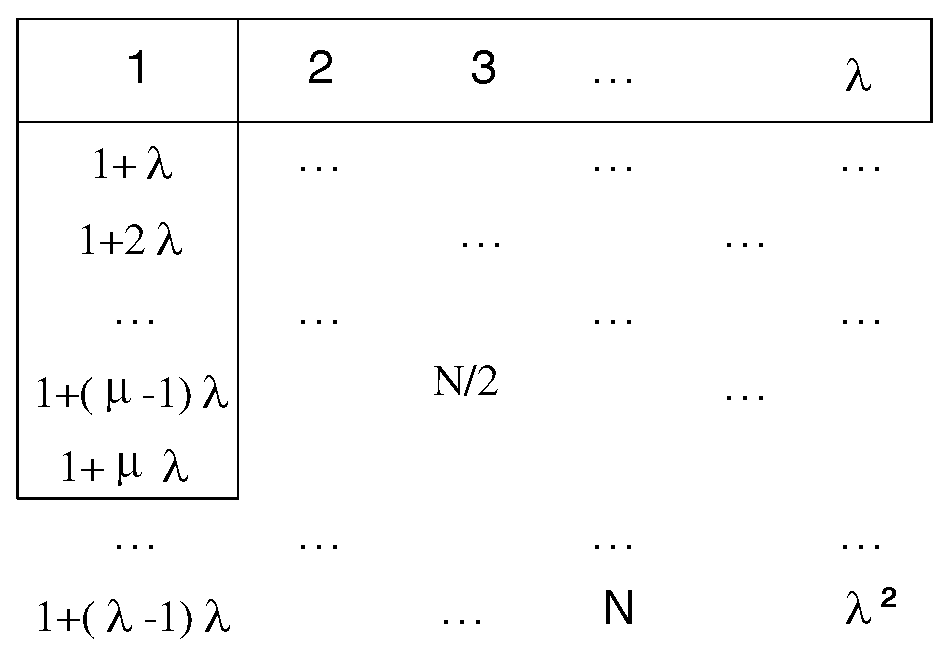
\includegraphics[width=2in]{./Figure/matrix}
\caption{An Sketch of RDS construction in Alg. \ref{RDS}}
\label{matrix}
\end{figure}


%The correctness proof of the construction
\begin{lemma}
\label{RDS1}
Set $R = \{r_0, r_1, ..., r_{\lambda + \mu - 1}\}$ constructed in Alg. \ref{RDS} is a RDS,
where $|R| = \lambda + \mu = \lceil \sqrt{N}  \rceil + \lceil \frac{\lceil \sqrt{N} \rceil}{2} \rceil
\approx \lceil \frac{3\sqrt{N}}{2}  \rceil$.
\end{lemma}


\begin{IEEEproof}
Obviously, if there exists one ordered pair $(a_i,a_j)$ satisfying  $a_i - a_j \equiv d$ (mod $N$),
an opposing pair $(a_j,a_i)$ exists such that
$a_j - a_i \equiv (N-d)$ (mod $N$). Thus we only need to find
at least one ordered pair $(a_i,a_j)$ for each $d \in [1, \lfloor N/2 \rfloor]$.

In the construction, $\lambda$ in Line \ref{RDSline1} is the smallest integer satisfying
$\lambda^2 \geq N$. Every $d$ within range $[1, \lfloor N/2 \rfloor]$
can be represented as: $ d = 1 + j \times \lambda - i$, where $1 \leq j \leq \mu,
1 \leq i \leq \lambda$. Thus, there exists $a_j = 1 + j \times \lambda$
from Line. \ref{RDSline2} and $a_i = i$ from Line. \ref{RDSline3}
satisfying  $a_j - a_i \equiv d$. Then, the lemma can be derived.
\end{IEEEproof}


%RDS Based Alano Algorithm
For symmetric nodes with duty cycle $\theta$, we present a RDS based Alano (RDS-Alano) algorithm as Alg. \ref{RDS-ND}.

In Alg. \ref{RDS-ND}, RDS is used to construct a deterministic
schedule for a node to turn on its radio in every period of length $T$,
and Alano is utilized as a probabilistic strategy to
determine whether it is in transmitting state or listening state.

\begin{algorithm}
\caption{RDS Based Alano Algorithm}
\label{RDS-ND}
\begin{algorithmic}[1]
\STATE $T := \lceil \frac{9}{4\theta^{2}} \rceil$; $t := 0$;
\STATE Invoke Alg. \ref{RDS} to construct the RDS $R = {r_0, r_1, ...,r_{\lceil \frac{3\sqrt{T}}{2}  \rceil}}$ under $Z_T$;
\WHILE {$True$}
   	 \IF{$(t + 1) \in R$}
    		\STATE Invoke Alg. \ref{Alano} to determine transmission state;
	\ELSE
    		\STATE Sleep;
	\ENDIF
	\STATE t := (t + 1) \% T;
\ENDWHILE
\end{algorithmic}
\end{algorithm}

%The time bound analysis   dutycycle zhengming

We derive discovery latency bound for RDS-Alano:

\begin{theorem}
\label{theoremRDS}
RDS-Alano guarantees that the discovery latency of a node
is bounded within $O(\frac{n\log n}{\theta^2})$ with high probability.
\end{theorem}

\begin{IEEEproof}
First, we verity that the duty cycle in RDS-Alano (denote as $\widetilde{\theta}$) is
$$
\widetilde{\theta} = \frac{|RDS|}{|T|} = \frac{\lceil \frac{3\sqrt{T}}{2}  \rceil}{T} = \theta.
$$

For any pair of neighbor nodes ($u_i$, $u_j$),
we can find an ordered pair ($r_i$, $r_j$) from their respective RDS
such that $r_i - r_j \equiv \delta_{ij}$ (mode $T$), where $\delta_{ij}$ is the time drift.
This implies any neighbor nodes can turn on their radios in the same time slot for at least once during every period of length $T$. 
Regarding each period of $T$ time slots as a `super' slot of Alano algorithm, we can derive that the discovery latency is bounded within $O(\frac{n\ln n}{\theta^2})$ slots with high probability by combining the analysis of Alano.
\end{IEEEproof}

\begin{remark}
In a RDS, a node can discovery its neighbors in different time slots. When treating a period of $T$ as a  `super' slot of Alano, 
there may be less than the total neighbors in each wake-up sub-slot,
resulting less collisions and lower latency compared to when all the neighbors wake up in the same sub-slot.
Thus the latency bound can not be larger.
\end{remark}


\subsection{TP-Alano for Asymmetric Nodes}


%Consider Local Duty Circle
Considering a more practical network where nodes can adjust their duty cycles, we present a traversing pointer method to synchronize time slots that nodes are in transmitting or listening state for asymmetric nodes.


For a more practical scenario, the nodes in a wireless sensor networks may be assigned to diverse tasks such as weather monitoring,
temperature measurement, etc., and thus ought to have asymmetric capability of
battery-management with local duty cycle $\theta_i$.

Suppose the duty cycle of node $u_i$ is $\theta_i$, we present a traversing pointer based Alano (TP-Alano) algorithm as Alg. \ref{P-ND}.
In each period of $T$ slots, a node turns on its radio in two different time slots, one of which is the
first slot of each period and the other one is a traversing slot that changes from period to period (as described in Line. \ref{P-NDline1}).

%Prime Based Neighbor Discovery Algorithm
\begin{algorithm}[!h]
\caption{Traversing Pointer Based Alano Algorithm}
\label{P-ND}
\begin{algorithmic}[1]
\STATE $T :=$ the smallest prime no less than $\frac{2}{\theta_i}$; $t := 0$;
\WHILE {$True$}
	\STATE $t_1 := t \% T$;
	\STATE $t_2 : =\lfloor t / T \rfloor \% (T - 1) +1$;\label{P-NDline1}
   	 \IF{$t_1 = 0~or~t_1 = t_2$}
    		\STATE Invoke Alg. \ref{Alano} to determine transmission state;
	\ELSE
    		\STATE Sleep;
	\ENDIF
	\STATE $t := t + 1$;
\ENDWHILE
\end{algorithmic}
\end{algorithm}

We call the first time slot of each period as \emph{fixed pointer} and the traversing
slot as \emph{traversing point}. The pointers are designed to guarantee that nodes $u_i, u_j$
could turn on their radio simultaneously in very period of length $T_i T_j$. A sketch of the pointers is described in Fig. \ref{TP}.

Note that, a period of $T$ slots is constructed as Line 1 where we try to \emph{find the smallest prime $\geq \frac{2}{\theta_i}$},
then it is likely to make the duty cycle of each period smaller than the expected one. This can be easily solved by selecting random slots to turn on the radio for listening in each period $T$, to conform to the expected duty cycle.


\begin{figure}[!h]
\centering
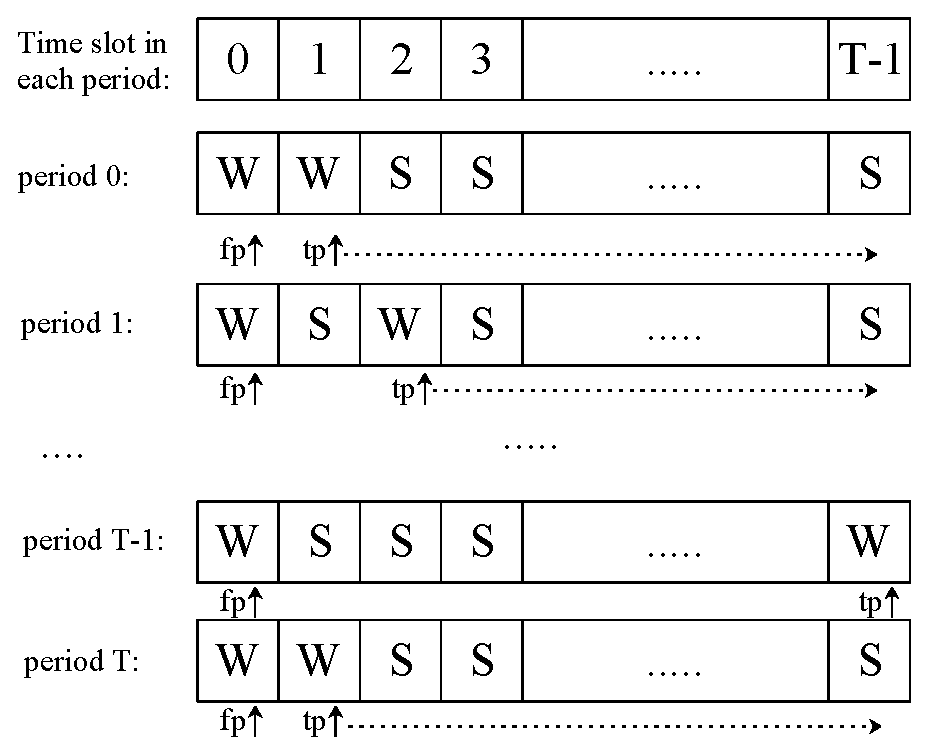
\includegraphics[width=2in]{./Figure/TP}
\caption{A sketch of TP construction in Alg. \ref{P-ND}}
\label{TP}
\end{figure}

%The correctness proof of the construction and the time bound analysis
We show the discovery latency of TP-Alano algorithm as:


\begin{theorem}
\label{PBND1}
TP-Alano guarantees that the discovery latency $L(i,j)$
is bounded within $O(\frac{nlogn}{\theta_i\theta_j})$ with high probability.,
where $\theta_i$ and $\theta_j$ are the duty cycles of
a pair of neighbors ($u_i$, $u_j$) respectively.
\end{theorem}



\begin{IEEEproof}
We first prove that any pair of nodes ($u_i$, $u_j$) turn on their radios (for transmitting or listening) simultaneously for at least once in every period of length $T_iT_j$.

\textbf{Case 1: $T_i \neq T_j$}. Since $T_i$ and $T_j$ are different primes,
according to Chinese Remainder Theorem\cite{ding1996chinese}, there exists a time slot $t_\tau \in \lbrack 0,T_iT_j ) $ satisfying:
\begin{equation}
\label{case1.1}
0 = t_\tau  \quad mod \quad  T_i.
\end{equation}
\begin{equation}
\label{case1.2}
\delta_{ij} = t_\tau  \quad mod \quad  T_j.
\end{equation}

Thus, there exists a fixed pointer of node $u_i$
and a fixed pointer of node $u_j$ in which both nodes turn on the radios in every period of length $T_iT_j$  .

\textbf{Case 2: $T_i = T_j$}. Since $T_i = T_j = T$, if the time drift between $u_i$ and $u_j$ is $\delta_{ij} = 0$, the fixed pointers of $u_i$ and $u_j$ will be the same in every period of length $T$.
Otherwise, since the traversing point will traverse all the time slots once during period of length $(T-1)T$,
there exists a traversing point of $u_i$ and a fixed pointer
of $u_j$ satisfying that both nodes turn on the radios simultaneously in every period of length $(T-1)T$; similarly a traversing point of $u_j$ and a fixed pointer of $i$ satisfying that they both turn on the radios.

Thus for any pair of neighbor nodes ($u_i$, $u_j$), they turn on their radios for transmitting or listening for at least once in every period of length $T_iT_j$. Considering
the whole period $T_iT_j$ to be a 'super' slot of Alano, we derive that the discovery latency is bounded within $O(\frac{n\ln n}{\theta_i\theta_j})$ with high probability.
\end{IEEEproof}






